\section{Referencial Teórico}
\label{sec:referencial-teorico}

Esta seção apresenta os conceitos fundamentais que embasam a pesquisa proposta, abordando arquiteturas de \textit{data lakes}, análise de dados em \textit{big data}, tecnologias de processamento distribuído e o roteamento de consultas utilizado no desenvolvimento do \textit{DyraSQL}. Os tópicos são organizados de forma a estabelecer o contexto teórico necessário para compreensão da solução proposta.

\subsection{Arquiteturas de \textit{Data Lake}}

\textit{Data lakes} representam repositórios centralizados que armazenam grandes volumes de dados em seu formato bruto, sem estruturação prévia, permitindo armazenamento escalável e flexível para diferentes tipos de análises \cite{dremiodatalake}. Diferentemente de \textit{data warehouses}, que organizam dados em esquemas estruturados pré-definidos, \textit{data lakes} mantêm dados em formato nativo, facilitando a ingestão de dados diversos e a exploração analítica posterior \cite{dremiodatalake}. Esta arquitetura é particularmente adequada para ambientes de \textit{big data}, nos quais o volume, variedade e velocidade dos dados tornam a estruturação prévia impraticável ou limitante \cite{ibmbigdata}.

A arquitetura de \textit{data lakes} baseada em armazenamento de objetos oferece escalabilidade e custos reduzidos de armazenamento, sendo que os dados são organizados em \textit{buckets} e objetos, permitindo acesso direto através de APIs \cite{dremiodatalake}. Esta abordagem elimina a necessidade de provisionamento prévio de capacidade, permitindo que organizações armazenem grandes volumes de dados de forma econômica \cite{ibmbigdata}. O \textit{DyraSQL} aproveita esta arquitetura para acessar metadados de tabelas \textit{Apache Iceberg} armazenadas em \textit{data lakes}, utilizando informações sobre volume e estrutura dos dados para tomada de decisões de roteamento. No protótipo local, o armazenamento de objetos é provido pelo MinIO, que expõe uma API compatível com sistemas de objetos utilizados em \textit{data lakes}.

\subsection{Análise de Dados em \textit{big data}}

A análise de dados em \textit{big data} envolve o processamento de volumes massivos de informações que excedem a capacidade de sistemas tradicionais de banco de dados, requerendo arquiteturas distribuídas e técnicas especializadas de processamento \cite{ibmbigdata}. Os desafios principais incluem o volume dos dados, a variedade de formatos e fontes, a velocidade de geração e a necessidade de extrair valor em tempo hábil para tomada de decisão \cite{ibmbigdata}. Sistemas de processamento distribuído, como Apache Spark e \textit{Trino}, viabilizam a análise de grandes volumes de dados através de paralelização e distribuição de carga de trabalho entre múltiplos nós computacionais \cite{apachespark2025,trinoconcepts}. O Apache Spark é um \textit{engine} unificado de análise para processamento de dados em larga escala, fornecendo APIs de alto nível e um \textit{engine} que suporta grafos de execução gerais \cite{apachespark2025}.

A eficiência na análise de \textit{big data} depende da escolha adequada da arquitetura de processamento, sendo que consultas leves podem ser executadas em \textit{clusters} menores, enquanto consultas complexas requerem infraestrutura com maior capacidade computacional \cite{ibmbigdata}. O \textit{DyraSQL} aborda este desafio através de roteamento dinâmico que direciona consultas para o \textit{cluster} mais adequado baseado em características dos dados e complexidade das operações, melhorando o custo-benefício do processamento.

\subsection{\textit{Trino}}

O \textit{Trino} é um \textit{engine} de consultas SQL distribuído projetado para consultar grandes volumes de dados armazenados em diversos sistemas, incluindo \textit{data lakes} baseados em armazenamento de objetos \cite{trinoconcepts}. A arquitetura do \textit{Trino} é baseada em um modelo de coordenação distribuída, sendo que um nó coordenador recebe consultas SQL e coordena a execução entre múltiplos nós trabalhadores (\textit{workers}), cada um processando uma porção dos dados em paralelo \cite{trinoconcepts}. Esta arquitetura permite escalabilidade horizontal através da adição de nós trabalhadores, aumentando a capacidade de processamento conforme a demanda cresce \cite{trinoconcepts}.

O \textit{Trino} suporta conectores para diversos sistemas de armazenamento, incluindo \textit{Apache Iceberg}, permitindo consultas SQL unificadas sobre dados armazenados em diferentes formatos e localizações \cite{trinoconcepts}. O \textit{DyraSQL} utiliza o \textit{Trino} como \textit{engine} de consultas, aproveitando sua capacidade de processamento distribuído e o suporte nativo a tabelas \textit{Apache Iceberg}. A integração com \textit{Trino Gateway} permite roteamento de consultas para diferentes \textit{clusters} de execução baseado em análise prévia de metadados \cite{trinogateway}. No ambiente experimental, o conector \textit{Iceberg} é configurado com catálogo REST, de modo que múltiplos \textit{clusters} compartilhem o mesmo catálogo e o mesmo \textit{warehouse} de objetos.

\subsection{Catálogo de Metadados}

Sistemas de consulta sobre \textit{data lakes} dependem de um catálogo que descreva esquemas, localização dos dados e estatísticas das tabelas, permitindo que o \textit{engine} descubra e acesse os dados sem conhecer a estrutura física dos arquivos \cite{apachehive2025}. O Apache Hive popularizou o \textit{Hive Metastore} como catálogo compartilhado entre ferramentas de análise \cite{apachehive2025}. O \textit{Apache Iceberg} admite diferentes implementações de catálogo, incluindo o \textit{Hive Metastore} e o catálogo REST, que expõe uma API HTTP para operações de metadados \cite{iceberg2024}.

O \textit{DyraSQL} não depende de um provedor específico de catálogo. O protótipo local utiliza o catálogo REST do \textit{Apache Iceberg} compartilhado pelos \textit{clusters} \textit{Trino}, garantindo consistência de metadados independentemente do \textit{cluster} selecionado para execução.

\subsection{\textit{Apache Iceberg}}
\label{sec:apache-iceberg}

O \textit{Apache Iceberg} é uma especificação de tabela para \textit{data lakes} que oferece capacidades avançadas de gerenciamento de dados, incluindo versionamento, \textit{schema evolution} e melhorias de consulta \cite{iceberg2024}. Sua arquitetura permite o armazenamento eficiente de metadados que podem ser utilizados para melhoria de consultas e tomada de decisões sobre processamento \cite{iceberg2024}. O \textit{Apache Iceberg} mantém uma estrutura hierárquica de metadados que oferece informações detalhadas sobre as tabelas, sendo que a Figura \ref{fig:iceberg-metadata} ilustra esta estrutura com os três níveis principais, arquivo de metadados (\textit{metadata}.json), lista de manifestos (\textit{manifest-list}) e arquivos de manifesto (\textit{manifest}) \cite{iceberg2024}. A especificação define que cada tabela possui um arquivo de metadados principal que contém informações sobre o esquema, partições, \textit{snapshots} e histórico de alterações, sendo que os manifestos listam os arquivos de dados que compõem cada \textit{snapshot}, incluindo estatísticas de colunas, contagens de registros e informações de partição \cite{iceberg2024}. Esta arquitetura permite que sistemas de consulta baseiem a execução em informações precisas sobre o volume e a distribuição dos dados, sendo essa camada de estatísticas por arquivo a origem dos valores que o comando \textit{EXPLAIN (TYPE IO)} do \textit{Trino} expõe de forma agregada, como \textit{outputSizeInBytes} e \textit{outputRowCount}, consumidos pelo \textit{DyraSQL} como entrada do Fator de volume descrito na Seção~\ref{sec:algoritmo-decisao}.

\begin{figure}[ht]
	\centering
	\caption{Estrutura de Metadados do \textit{Apache Iceberg}}
	\label{fig:iceberg-metadata}
	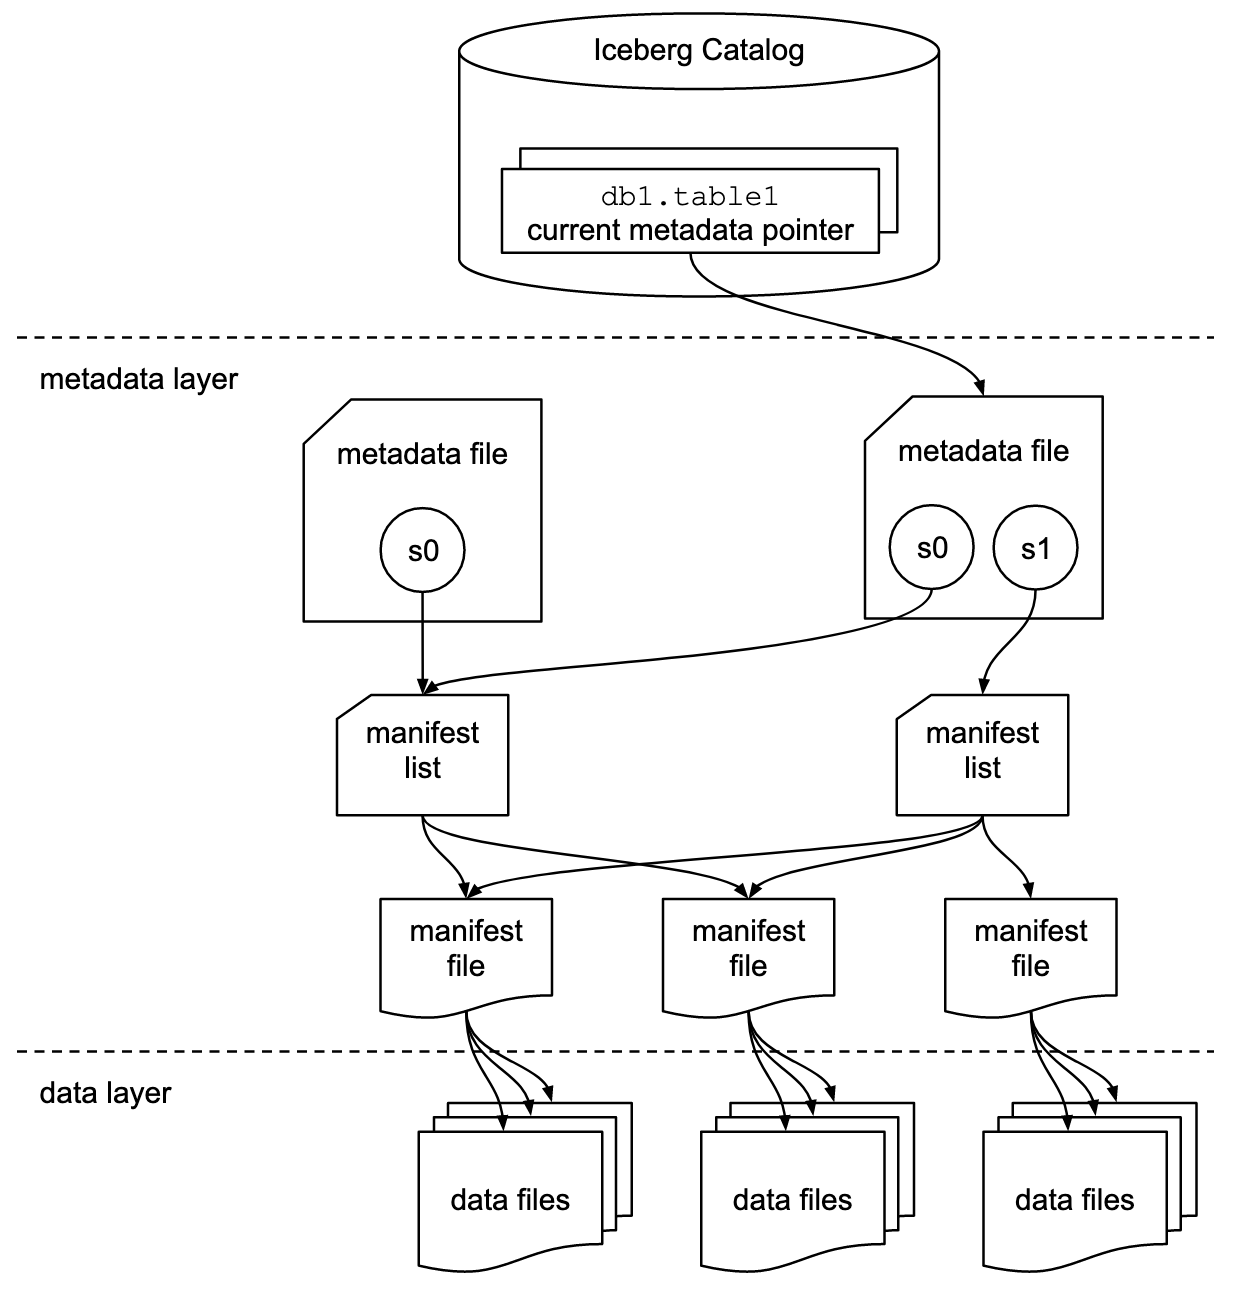
\includegraphics[width=0.8\textwidth]{figuras/iceberg-metadata.png}\\
	\fonte{\cite{iceberg2024}.}
\end{figure}
\FloatBarrier

A Figura \ref{fig:iceberg-metadata} demonstra a estrutura hierárquica de metadados do \textit{Apache Iceberg}, evidenciando como os três níveis principais organizam informações sobre volume, estrutura e distribuição dos dados. Esta organização facilita a extração de metadados relevantes para tomada de decisões de roteamento no \textit{DyraSQL}.

\subsection{Processamento em \textit{clusters}}

A execução de consultas SQL em \textit{data lakes} ocorre tipicamente em \textit{clusters} de processamento com capacidades distintas de memória, paralelismo e tempo máximo de consulta. Consultas leves, com volume reduzido e poucas operações, podem ser atendidas por \textit{clusters} menores, com menor consumo de recursos. Consultas intermediárias demandam paralelismo moderado. Consultas pesadas, com grande volume de dados ou elevada complexidade, requerem \textit{clusters} mais robustos \cite{trinoconcepts,ibmbigdata}.

O \textit{DyraSQL} adota três faixas de capacidade, \textit{cluster small}, \textit{cluster medium} e \textit{cluster large}, implementadas no ambiente local como três instâncias \textit{Trino} com limites distintos de memória e tempo de execução. A classificação em faixas permite que o algoritmo de pontuação selecione o ambiente antes da execução, evitando tanto a subutilização de infraestrutura robusta em consultas simples quanto a saturação de \textit{clusters small} em consultas pesadas.

\subsection{Roteamento Dinâmico de Consultas}

O roteamento dinâmico de consultas envolve a seleção automática do ambiente de execução mais adequado baseado em características da consulta e dos dados, sendo uma abordagem explorada em diversos contextos para melhoria de recursos computacionais. Trabalhos recentes têm demonstrado a importância de execução adaptativa e robusta de consultas em ambientes de \textit{data lakehouse} \cite{xue2024}, sendo que abordagens baseadas em modelos de custo aprendidos \cite{strausz2025} e elasticidade em tempo de execução \cite{zhang2025} têm sido exploradas para melhoria de custo-benefício. O \textit{DyraSQL} implementa roteamento dinâmico baseado em análise prévia de metadados de tabelas \textit{Apache Iceberg}, direcionando consultas para \textit{clusters small}, \textit{medium} ou \textit{large} com base em volume de dados, complexidade da consulta e histórico de execuções similares.
